\documentclass[compress]{beamer}
\usepackage{ifthen,verbatim}

\title{ME1/1 Reconstruction Issues Seen in CSA08 Alignment}
\author{Jim Pivarski, Alexei Safonov, K\'aroly Banicz$^*$}
\institute{Texas A\&M University, $^*$FermiLab}
\date{22 May, 2008}

\newcommand{\isnote}{}
\xdefinecolor{lightyellow}{rgb}{1.,1.,0.25}
\xdefinecolor{darkblue}{rgb}{0.1,0.1,0.7}

%% Uncomment this to get annotations
%% \def\notes{\addtocounter{page}{-1}
%%            \renewcommand{\isnote}{*}
%% 	   \beamertemplateshadingbackground{lightyellow}{white}
%%            \begin{frame}
%%            \frametitle{Notes for the previous page (page \insertpagenumber)}
%%            \itemize}
%% \def\endnotes{\enditemize
%% 	      \end{frame}
%%               \beamertemplateshadingbackground{white}{white}
%%               \renewcommand{\isnote}{}}

%% Uncomment this to not get annotations
\def\notes{\comment}
\def\endnotes{\endcomment}

\setbeamertemplate{navigation symbols}{}
\setbeamertemplate{headline}{\mbox{ } \hfill
\begin{minipage}{5.5 cm}
\vspace{-0.75 cm} \small
\end{minipage} \hfill
\begin{minipage}{4.5 cm}
\vspace{-0.75 cm} \small
\begin{flushright}
\ifthenelse{\equal{\insertpagenumber}{1}}{}{Jim Pivarski \hspace{0.2 cm} \insertpagenumber\isnote/\pageref{numpages}}
\end{flushright}
\end{minipage}\mbox{\hspace{0.2 cm}}\includegraphics[height=1 cm]{../cmslogo} \hspace{0.1 cm} \includegraphics[height=1 cm]{../tamulogo} \hspace{0.01 cm} \vspace{-1.05 cm}}

\begin{document}
\frame{\titlepage}

%% \begin{notes}
%% \item This is the annotated version of my talk.
%% \item If you want the version that I am presenting, download the one
%% labeled ``slides'' on Indico (or just ignore these yellow pages).
%% \item The annotated version is provided for extra detail and a written
%% record of comments that I intend to make orally.
%% \item Yellow notes refer to the content on the {\it previous} page.
%% \item All other slides are identical for the two versions.
%% \end{notes}

\begin{frame}
\begin{itemize}\setlength{\itemsep}{0.75 cm}
\item Working on the iCSA08 alignment exercise, I found two strange features in ME1/1 residuals in CMSSW\_2\_0\_7
\item It doesn't jeopardize the alignment
\item But it's something that should be made known, if it is not already
\end{itemize}
%% \hspace{-0.83 cm} \textcolor{darkblue}{\Large Outline2}
\end{frame}

\begin{frame}
\frametitle{ME1/1a $y$ ``residual'' asymmetry}
\small
\begin{itemize}
\item These ``residuals'' are the distance between a track extrapolated from the tracker to the muon hit (track $y$ position minus hit)
\item They are not with respect to a best-fit track to the muon hits
\item That's why the distribution is wide, but unbiased by the hit
\item Note the high-side tail, in 1\_6\_7 and 2\_0\_7
\end{itemize}

\begin{columns}
\column{0.5\linewidth}
\mbox{ } \hfill CMSSW\_1\_6\_7

\mbox{ } \hfill 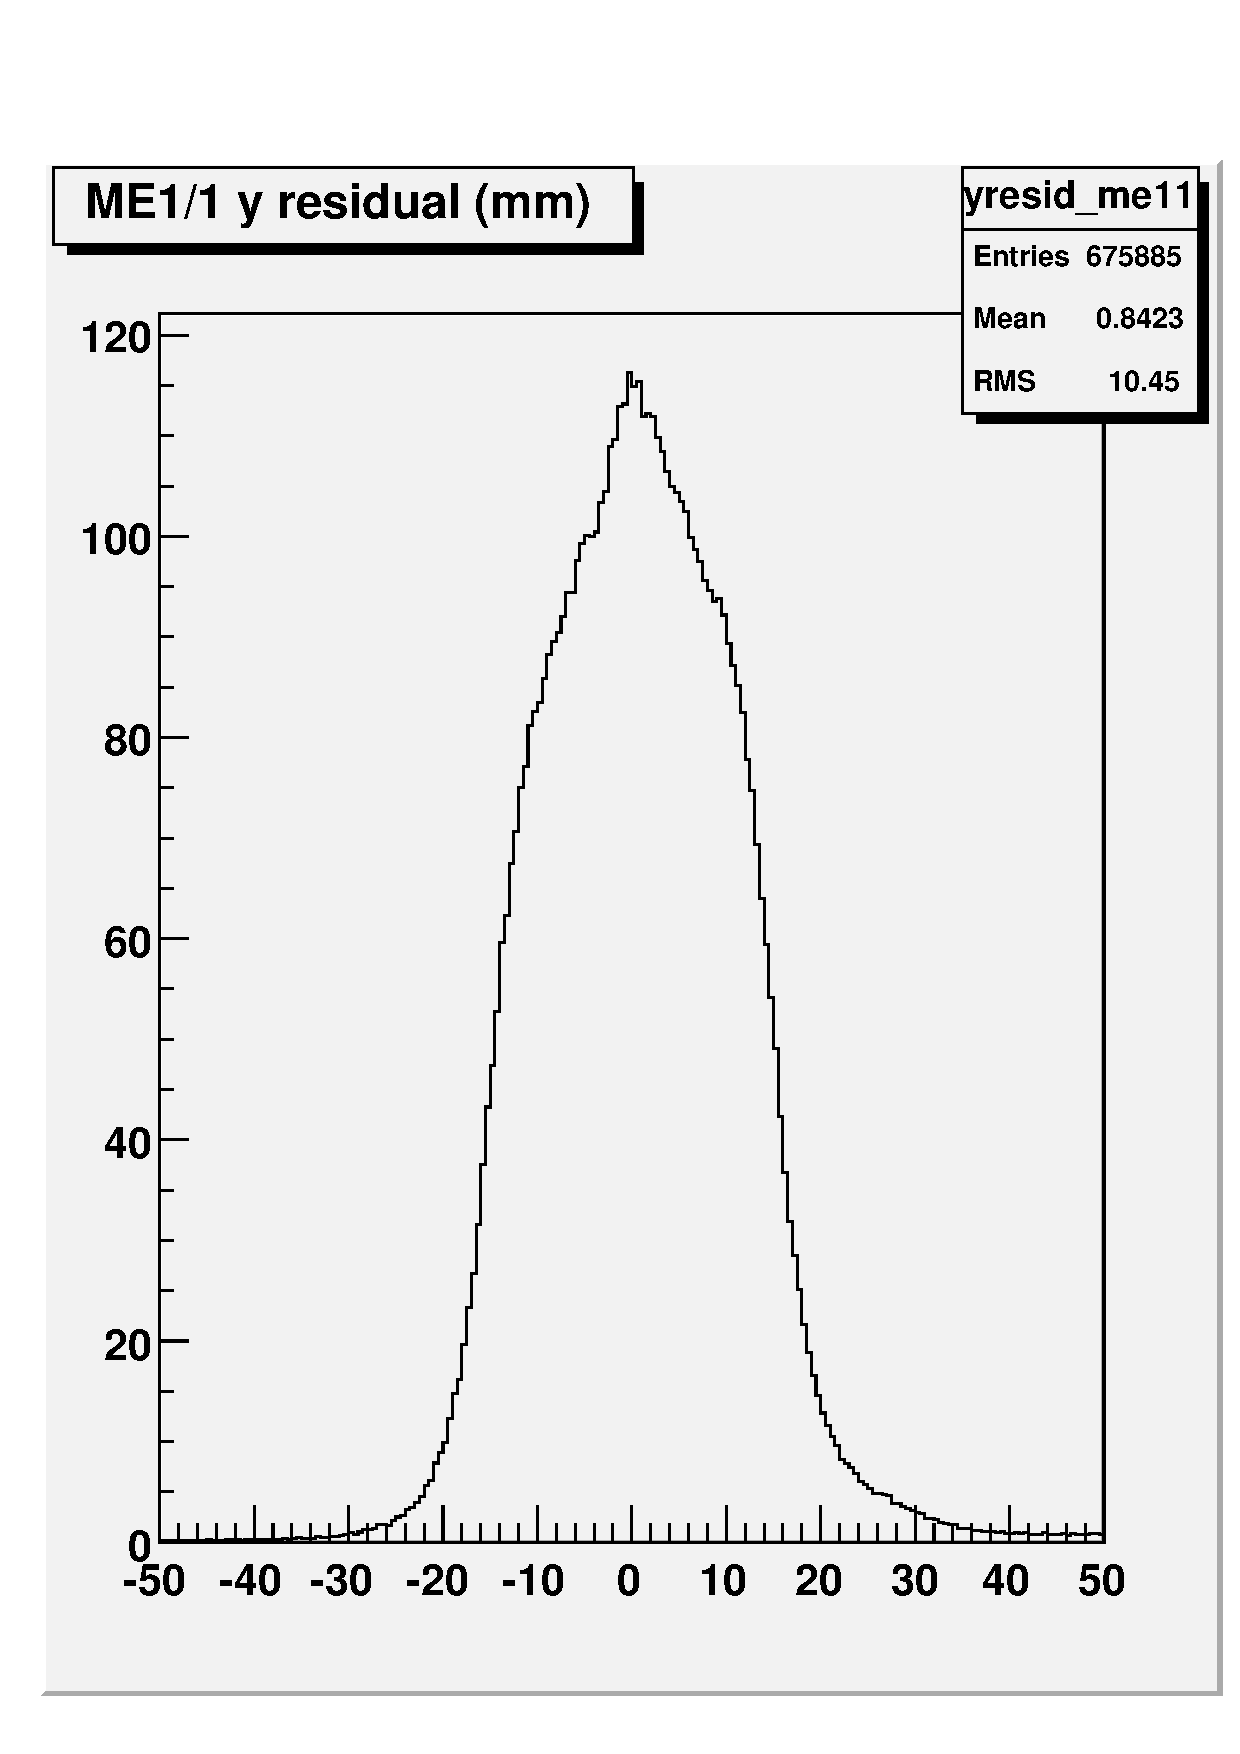
\includegraphics[width=0.7\linewidth]{talk_me11_yresid_167.pdf}
\column{0.5\linewidth}
CMSSW\_2\_0\_7

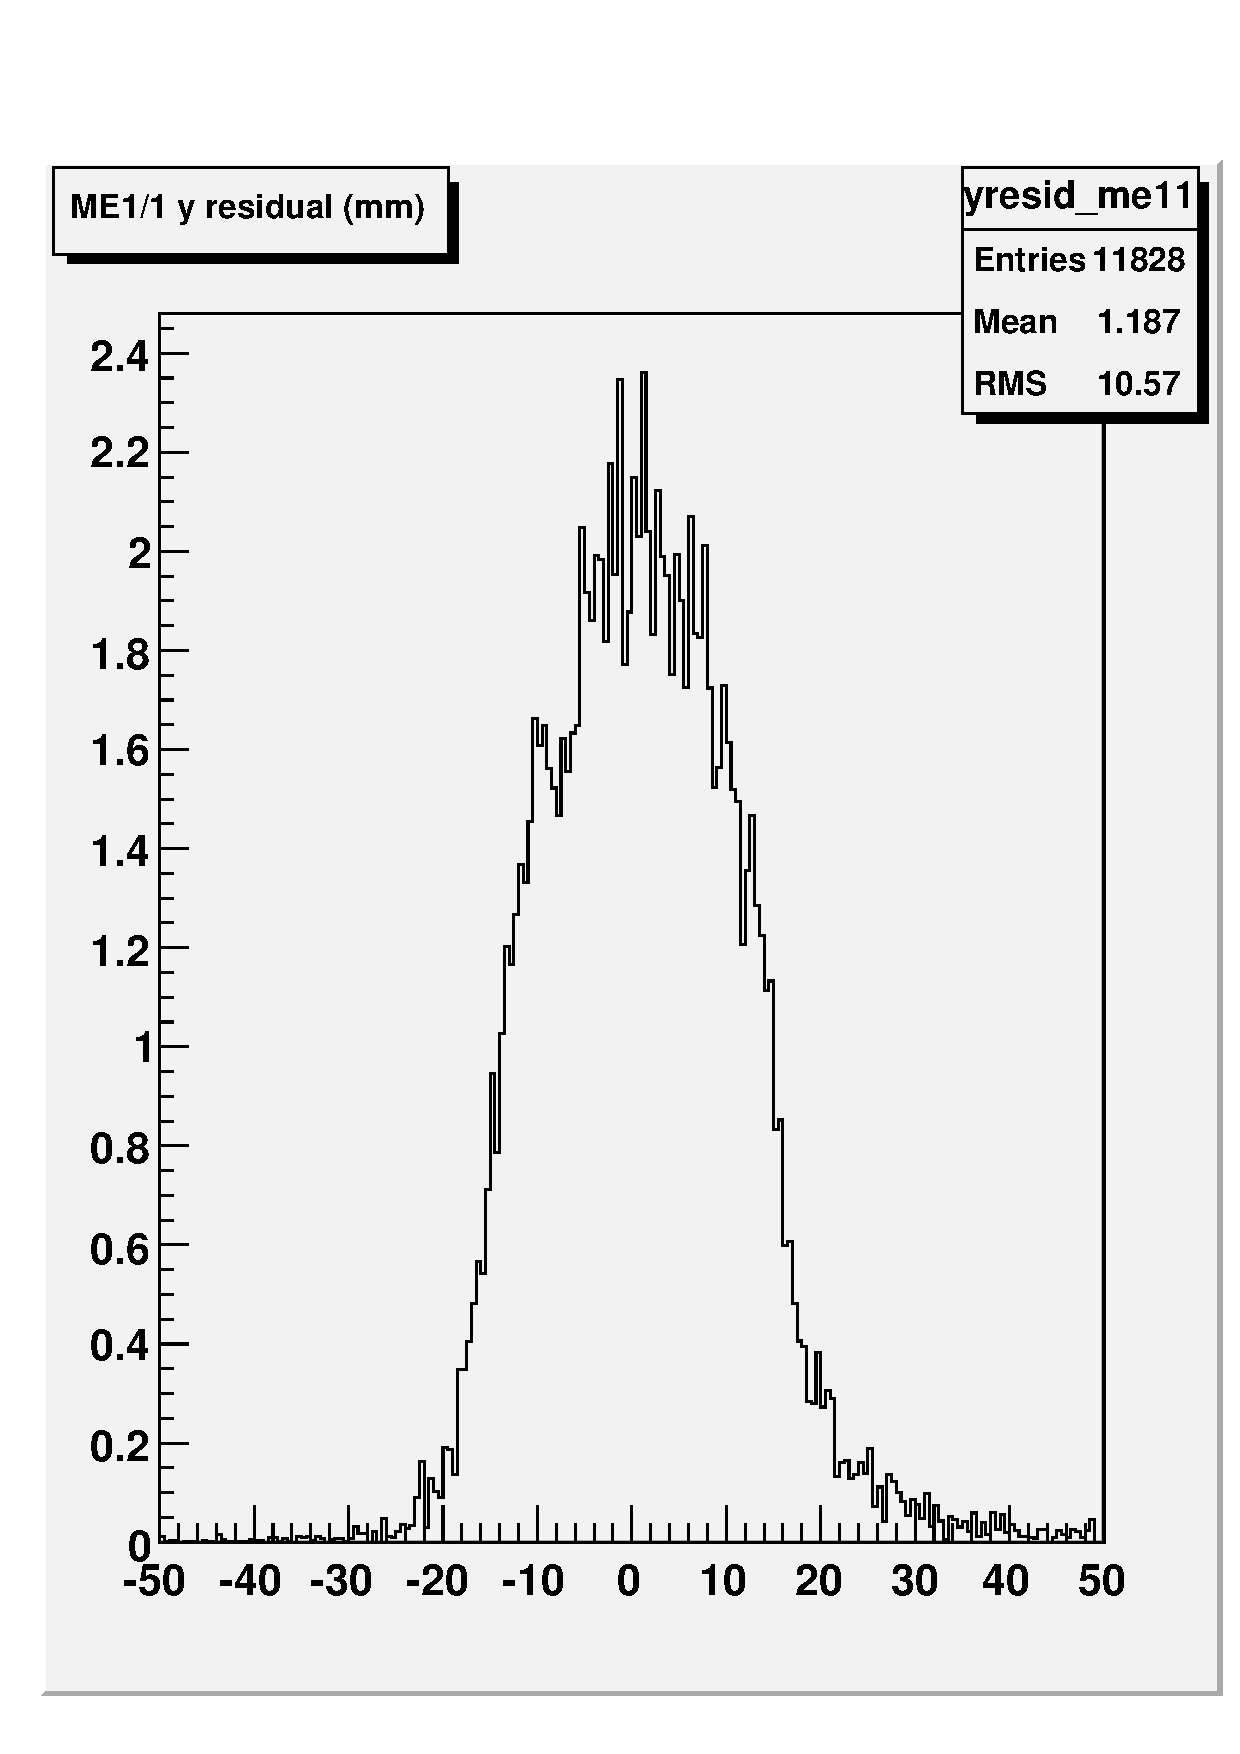
\includegraphics[width=0.7\linewidth]{talk_me11_yresid_207.pdf}
\end{columns}
\end{frame}

\begin{frame}
\frametitle{ME1/1a $y$ asymmetry}
\small

\begin{itemize}
\item The high-side tail is on every chamber (I checked individually);
you can see that the $y$ residual means of each chamber (histogrammed
below) are offset from zero
\item This is with ideal geometry (tracker and muon system)
\end{itemize}

\begin{columns}
\column{0.5\linewidth}
\mbox{ } \hfill CMSSW\_1\_6\_7

\mbox{ } \hfill 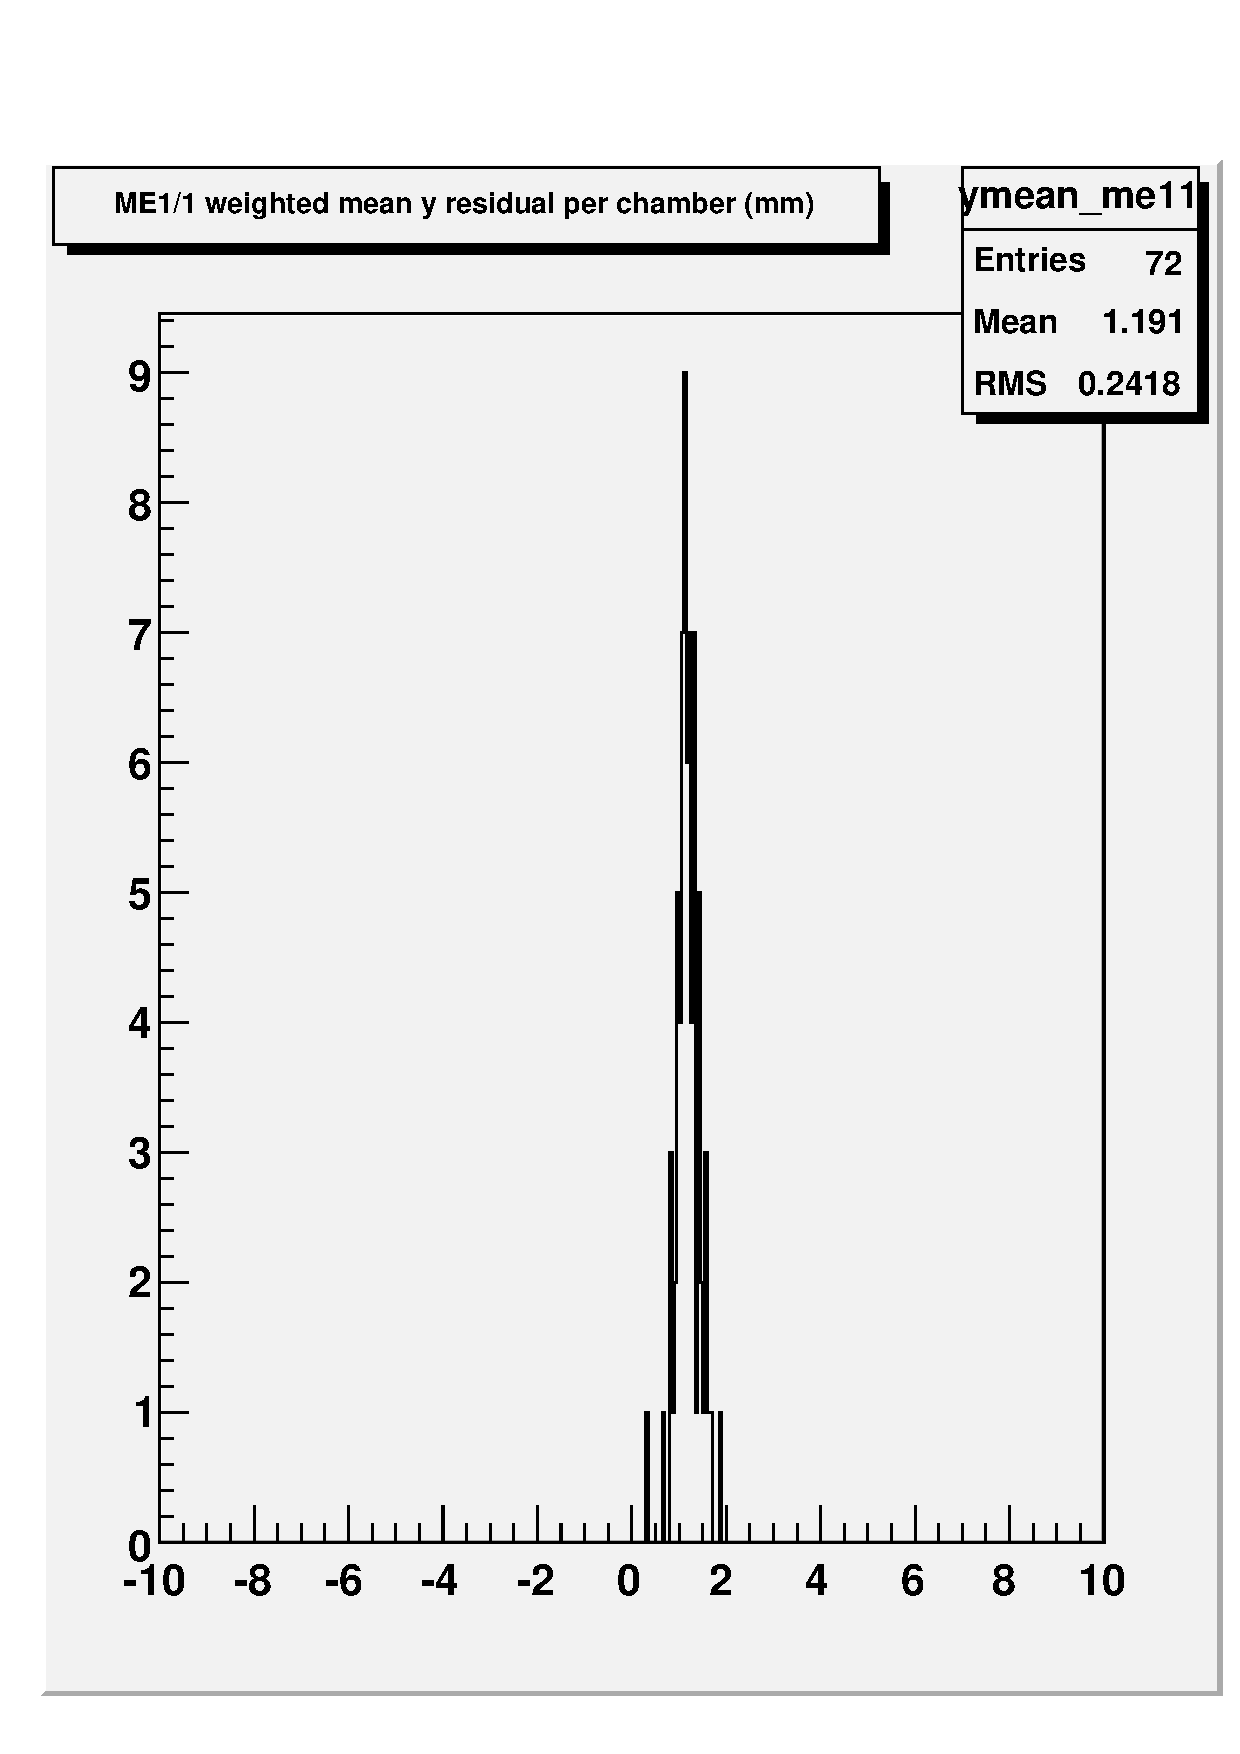
\includegraphics[width=0.7\linewidth]{talk_me11_ymean_167.pdf}
\column{0.5\linewidth}
CMSSW\_2\_0\_7

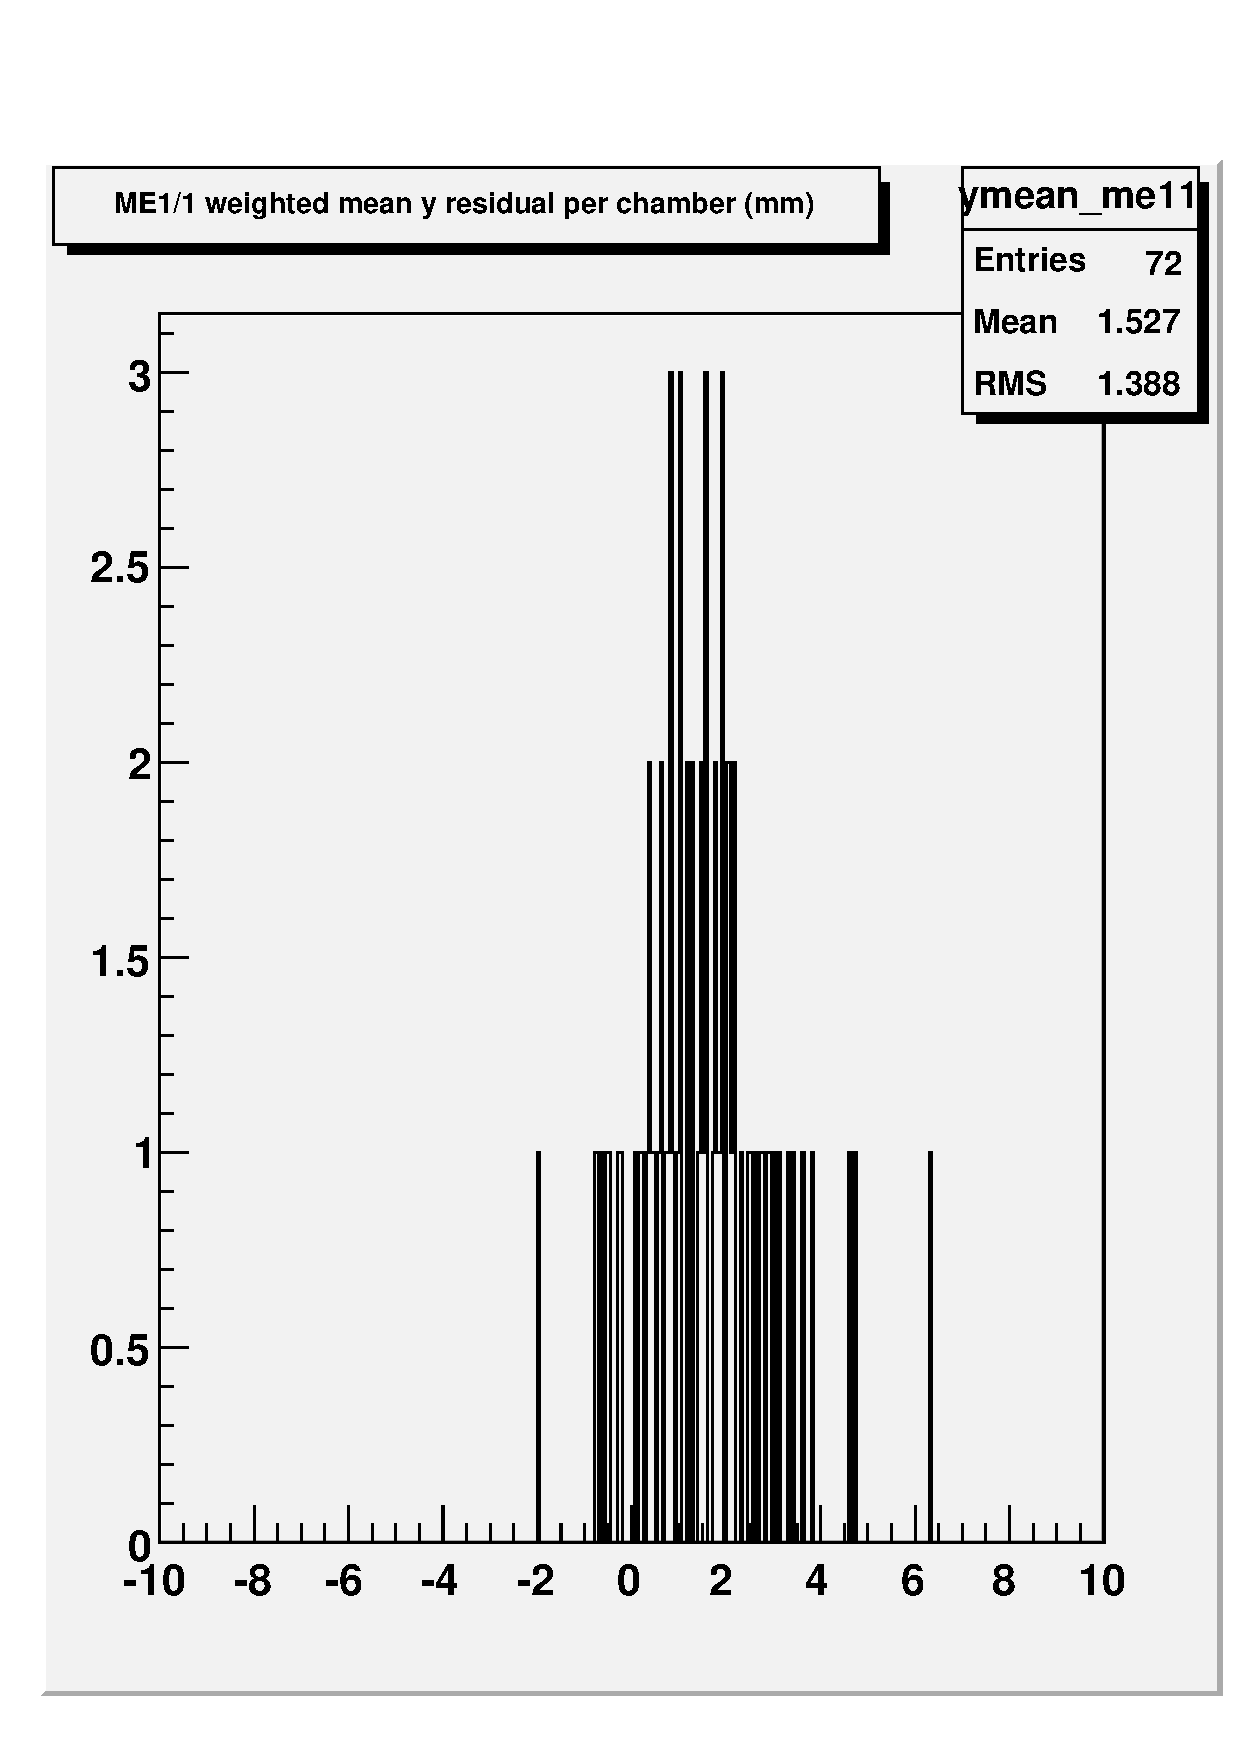
\includegraphics[width=0.7\linewidth]{talk_me11_ymean_207.pdf}
\end{columns}
\end{frame}

\begin{frame}
\frametitle{ME1/1b efficiency}
\small

\begin{itemize}
\item There's a new problem with efficiency on ME1/1b
\item The 2\_0\_7 subsample shown below has 11,828 hits on ME1/1a, but 21 hits on ME1/1b
\item This was not present in 1\_6\_7
\end{itemize}

\begin{columns}
\column{0.5\linewidth}
\mbox{ } \hfill CMSSW\_1\_6\_7

\mbox{ } \hfill 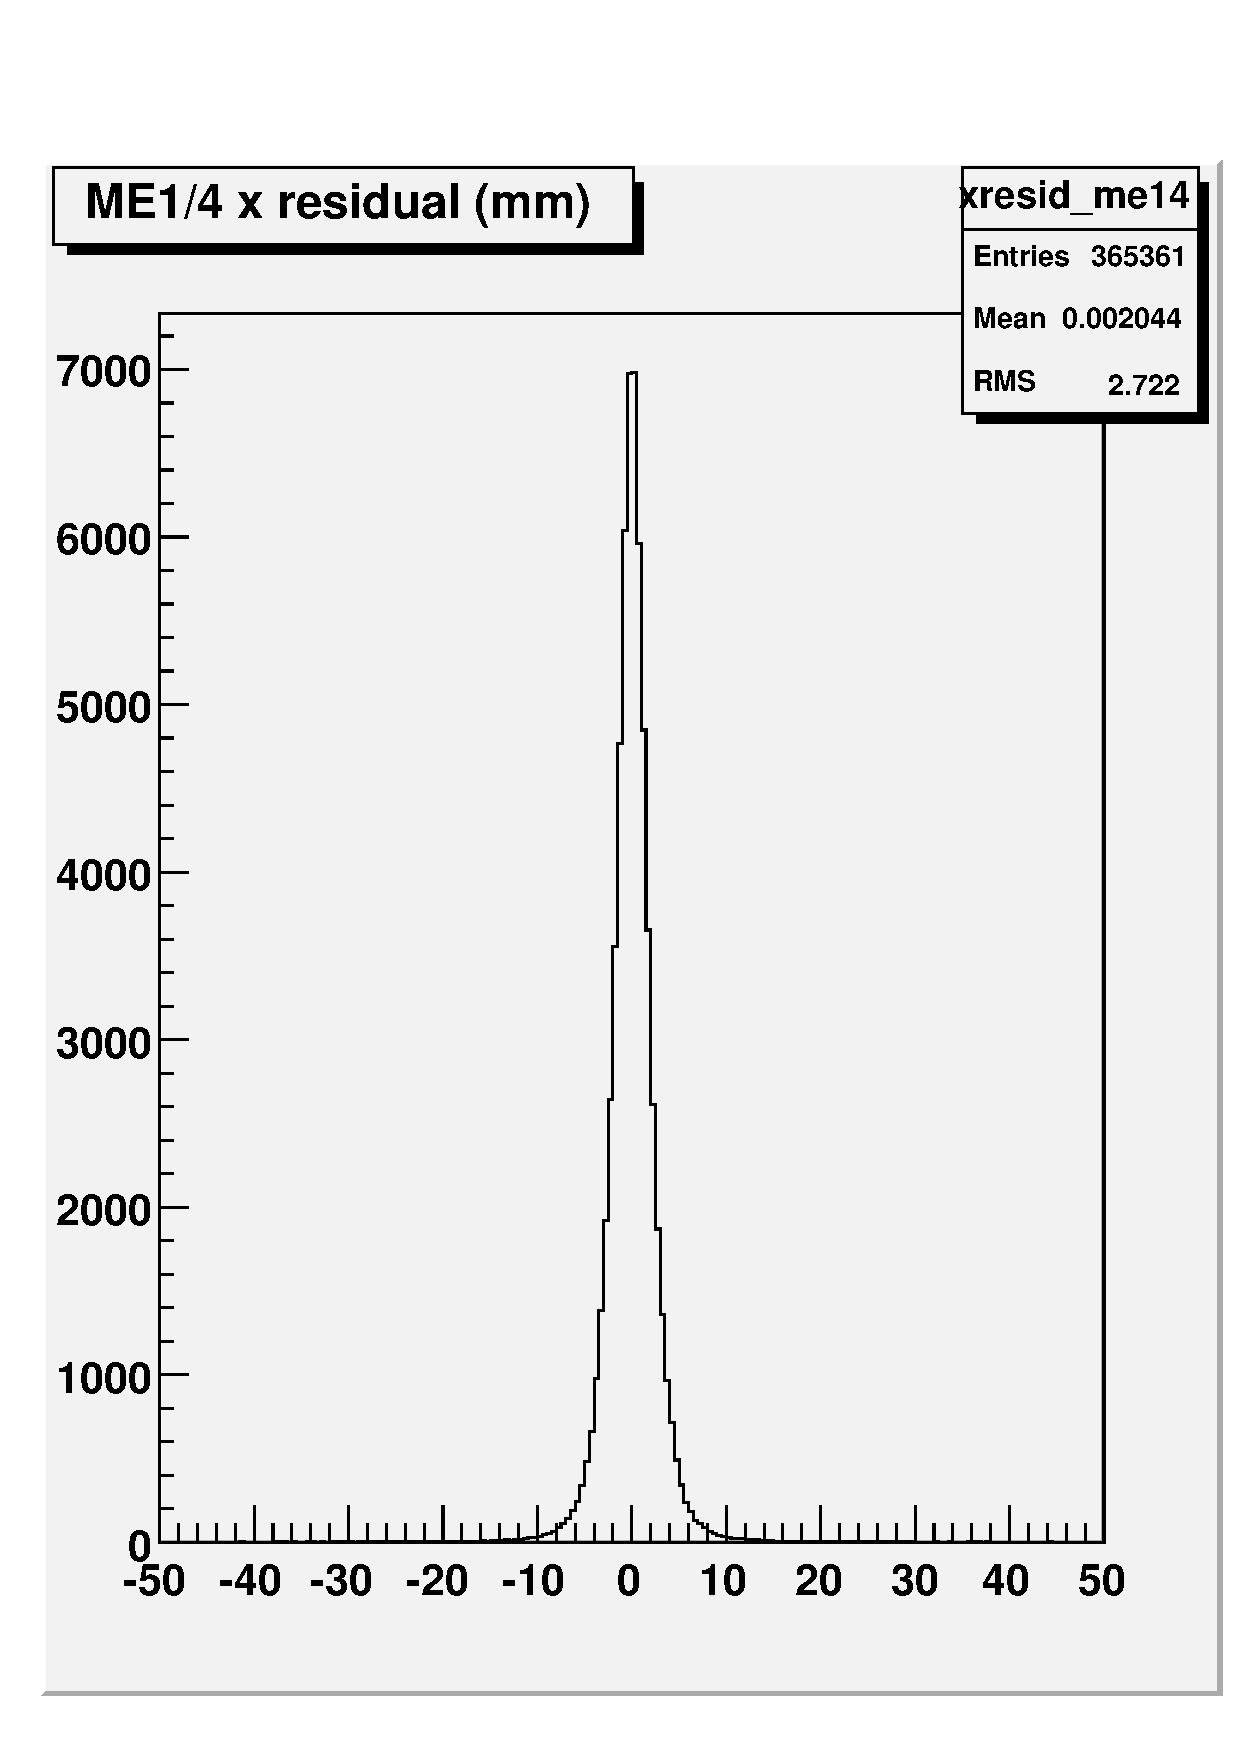
\includegraphics[width=0.7\linewidth]{talk_me14_xresid_167.pdf}
\column{0.5\linewidth}
CMSSW\_2\_0\_7

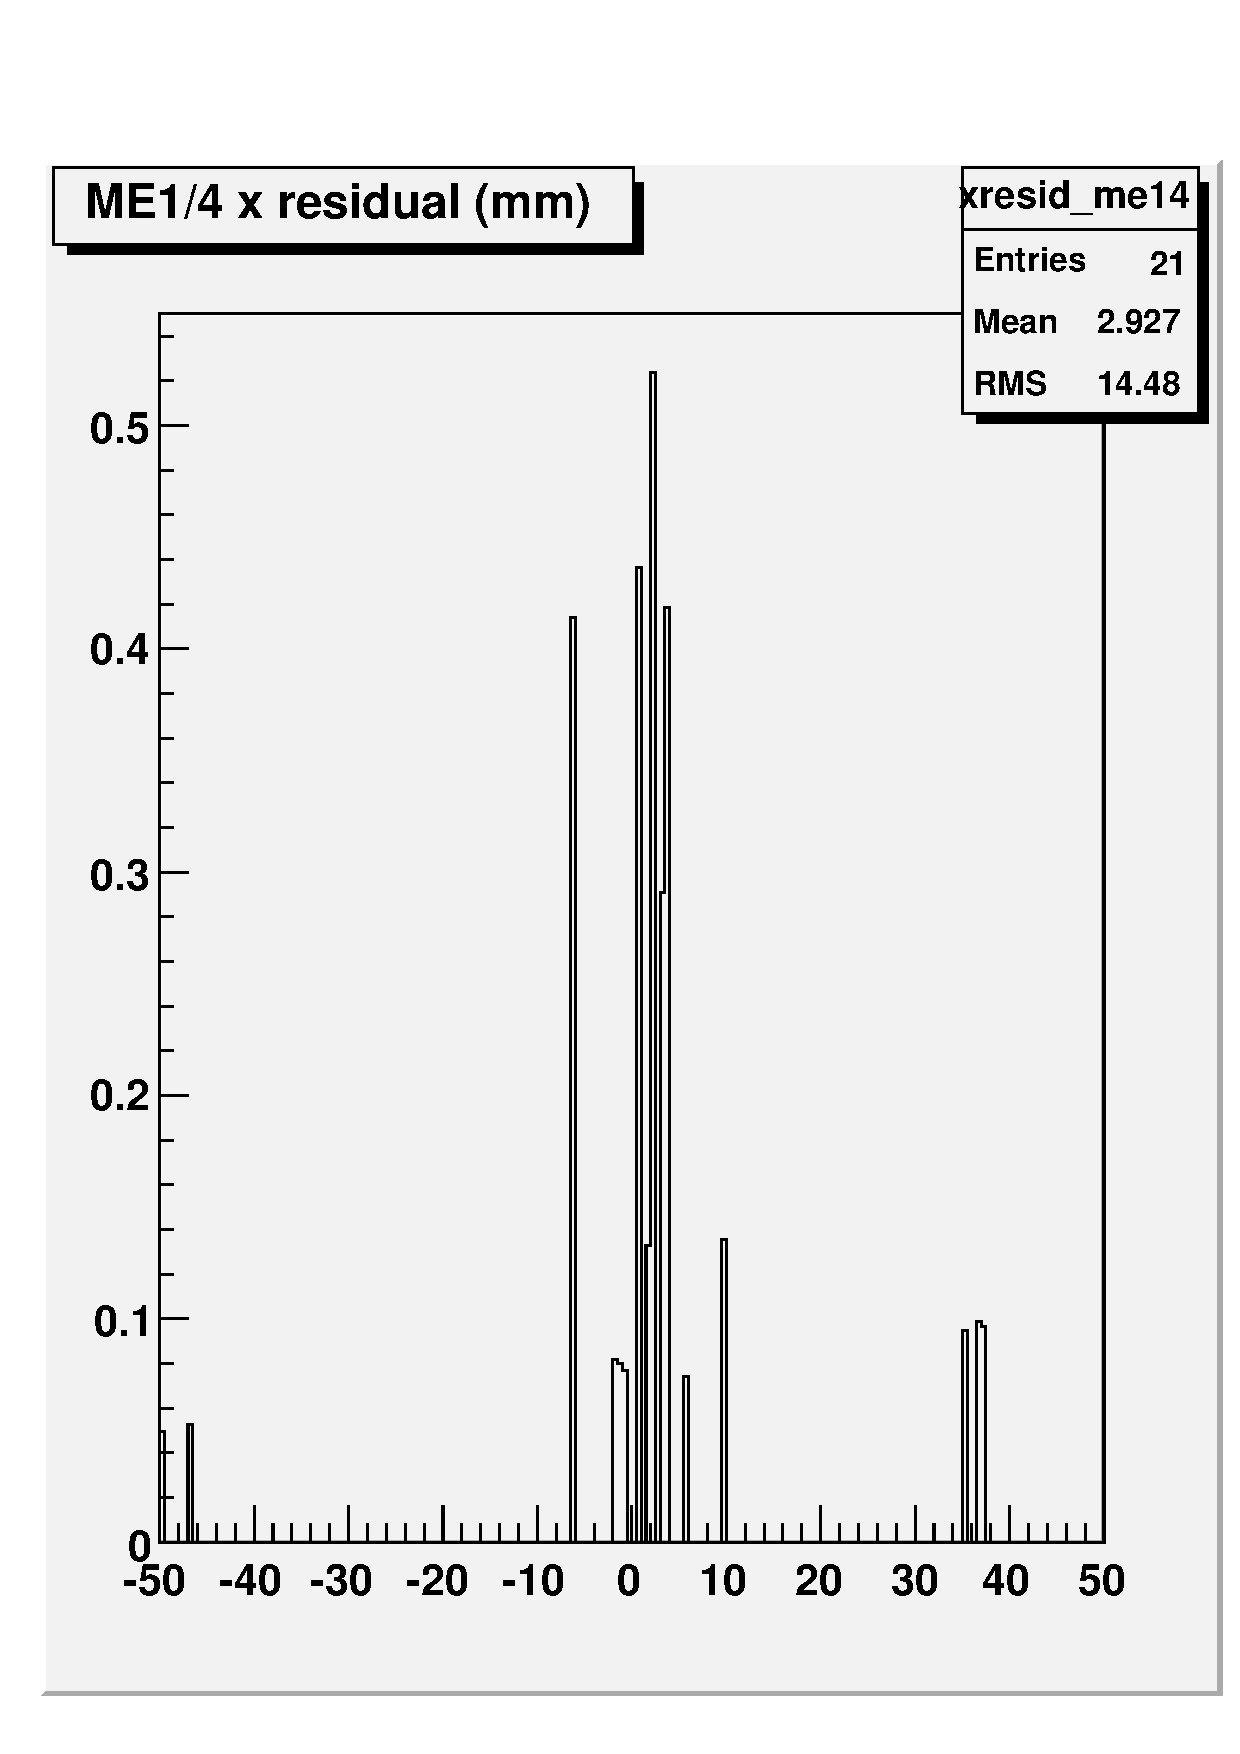
\includegraphics[width=0.7\linewidth]{talk_me14_xresid_207.pdf}
\end{columns}
\end{frame}



%% \section*{First section}
%% \begin{frame}
%% \begin{center}
%% \Huge \textcolor{blue}{First section}
%% \end{center}
%% \end{frame}

\begin{frame}
\frametitle{Conclusions}

\begin{itemize}\setlength{\itemsep}{0.75 cm}
\item None; I just wanted to make these two points!
\item Thanks!
\end{itemize}

\label{numpages}
\end{frame}

\end{document}
